\section{Experiments and Results}

% \uselengthunit{in}\printlength{\textwidth} = 4.8041 in
% \uselengthunit{mm}\printlength{\textwidth} = 121.99854 mm

To allow for a direct comparison with state-of-the-art lesion segmentation
methods, we evaluated our method on the FLAIR, T1-, and T2-weighted MRIs of the
20 publicly available labeled cases from the MS lesion segmentation challenge
2008 \cite{styner20083d}, which we downsampled from the original isotropic voxel
size of \SI{0.5}{\cubic\milli\metre} to an isotropic voxel size of
\SI{1.0}{\cubic\milli\metre}. In addition, we evaluated our method on an
in-house data set from an MS clinical trial of 500 subjects split equally into
training and test sets. The images were acquired from 45 different scanning
sites. For each subject, the data set contains T2- and PD-weighted MRIs with a
voxel size of \SI{0.937x0.937x3.000}{\milli\metre}. The main preprocessing steps
included rigid intra-subject registration, brain extraction, intensity
normalization, and background cropping.

We used a CEN with 32 filters and filter sizes of \num{9x9x9} and \num{9x9x5}
voxels for the challenge and in-house data sets, respectively. Training on a
single GeForce GTX 780 graphics card took between 6 and 32 hours per model
depending on the training set size. However, once the network is trained,
segmentation of trimodal 3D volumes with a resolution of, e.g.,
\num{159x201x155} voxels can be performed in less than one second. As a
rough\footnote{Ciresan et al. used a more complex network that is composed of 11
layers. However, their network was trained on much smaller images, which roughly
compensates for the increased complexity.} comparison, Ciresan et al.
\cite{Ciresan2012} reported that their patch-based method required 10 to 30
minutes to segment a single 2D image with a resolution of \num{512x512} voxels
using four graphics cards, which demonstrates the large speed-ups gained by
processing entire volumes.

\begin{figure}[tb]
\centering
\small
\def\MRIwidth{0.15\textwidth}

\begin{tikzpicture} 
\tikzstyle{leftlabel}=[rotate=90, align=center,overlay,above]

\matrix [matrix of nodes, nodes={anchor=center, inner sep=1pt}] {
        &[4pt] FLAIR & T1w & T2w & Ground truth & Our method \\[4pt]
\node[leftlabel] {CHB\,07\\(DSC\,=\,\SI{60.58}{\percent})}; &
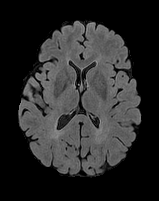
\includegraphics[width=\MRIwidth]{figures/CHB07-FLAIR-s88} &
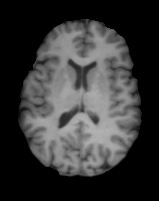
\includegraphics[width=\MRIwidth]{figures/CHB07-T1w-s88} &
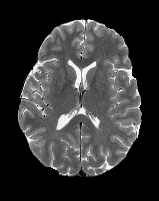
\includegraphics[width=\MRIwidth]{figures/CHB07-T2w-s88} &
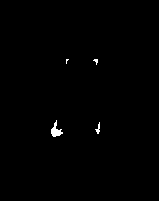
\includegraphics[width=\MRIwidth]{figures/CHB07-gold-s88} &
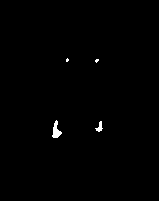
\includegraphics[width=\MRIwidth]{figures/CHB07-pred-s88} \\
\node[leftlabel] {CHB\,04\\(DSC\,=\,\SI{61.37}{\percent})}; &
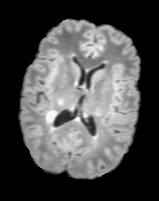
\includegraphics[width=\MRIwidth]{figures/CHB04-FLAIR-s85} &
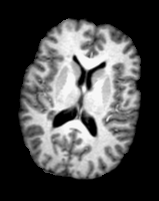
\includegraphics[width=\MRIwidth]{figures/CHB04-T1w-s85} &
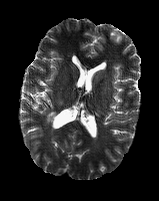
\includegraphics[width=\MRIwidth]{figures/CHB04-T2w-s85} &
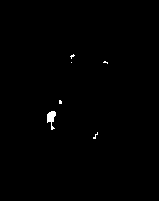
\includegraphics[width=\MRIwidth]{figures/CHB04-gold-s85} &

\includegraphics[width=\MRIwidth]{figures/CHB04-pred-s85} \\
\node[leftlabel] {UNC\,09\\(DSC\,=\,\SI{9.01}{\percent})}; &
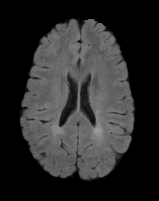
\includegraphics[width=\MRIwidth]{figures/UNC09-FLAIR-s89} &
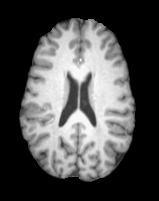
\includegraphics[width=\MRIwidth]{figures/UNC09-T1w-s89} &
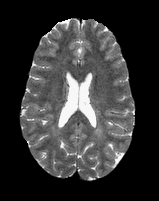
\includegraphics[width=\MRIwidth]{figures/UNC09-T2w-s89} &

\includegraphics[width=\MRIwidth]{figures/UNC09-gold-s89} &
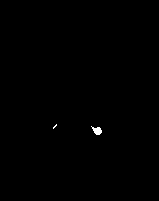
\includegraphics[width=\MRIwidth]{figures/UNC09-pred-s89} \\
};
\end{tikzpicture}

\caption{Example segmentations of our method for three different subjects from
the challenge data set. Our method performed well and consistently despite the
large contrast differences seen between the first two rows. In the third row,
our method also segmented lesions that have similar contrast, but these regions
had not been identified as lesions by the manual rater, which highlights the
difficulty in distinguishing focal lesions from diffuse damage, even for
experts.}

\label{fig:segmentation}
\end{figure}

We evaluated our method on the challenge data set using 5-fold
cross-valida\-tion and calculated the true positive rate (TPR), positive
predictive value (PPV), and Dice similarity coefficient (DSC) between the
predicted segmentations and the resampled ground truth.
Figure~\ref{fig:segmentation} shows a comparison of three subjects from the
challenge data set. The first two rows show the FLAIR, T1w, T2w, ground truth
segmentations, and predicted segmentations of two subjects with a DSC of
\SI{60.58}{\percent} and \SI{61.37}{\percent}. Despite the large contrast
differences between the two subjects, our method performed well and
consistently, which indicates that our model was able to learn features that are
robust to a large range of intensity variations. The last row shows a subject
with a DSC of \SI{9.01}{\percent}, one of the lowest DSC scores from the data
set. Our method segmented lesions that have similar contrast to the other two
subjects, but these regions were not classified as lesions by the manual rater.
This highlights the difficulty of manual lesion segmentation, as the difference
between diffuse white matter pathology and focal lesions is often indistinct. A
quantitative comparison of our method with other state-of-the-art methods is
summarized in Table~\ref{tab:state}. Our method outperforms the winning method
(Souplet et al. \cite{souplet2008}) of the MS lesion segmentation challenge 2008
and the currently best unsupervised method reported on that data set (Weiss et
al. \cite{weiss2013}) in terms of mean TPR and PPV. Our method performs
comparably to a current method (Geremia et al. \cite{geremia2010}) that uses a
carefully designed set of features specifically designed for lesion
segmentation, despite our method having learned its features solely from a
relatively small training set.

\begin{table}[tb]
\def\tabspace{12pt}

\caption{Comparison of our method with state-of-the-art lesion segmentation
methods in terms of mean TPR, PPV, and DSC. Our method performs comparably to
the best methods reported on the MS lesion segmentation challenge data set.}

\label{tab:state}
\centering
\begin{tabular}{l%
@{\hspace{\tabspace}}S[table-format=2.2]
@{\hspace{\tabspace}}S[table-format=2.2]
@{\hspace{\tabspace}}S[table-format=2.2]
}
\toprule
Method & {TPR} & {PPV} & {DSC} \\ 
\midrule
Souplet et al. \cite{souplet2008} & 20.65 & 30.00 & {---} \\ 
Weiss et al. \cite{weiss2013} & 33.00 & 36.85 & 29.05 \\ 
Geremia et al. \cite{geremia2010} & 39.85 & 40.35 & {---}  \\
Our method & 39.71 & 41.38 & 35.52 \\
\bottomrule
\end{tabular}
\end{table}

To evaluate the impact of the training set size on the segmentation performance,
we trained our model on our in-house data set with a varying number of training
samples and calculated the mean DSC on the training and test sets as illustrated
in Fig.~\ref{fig:bioms}. For small training sets, there is a large difference
between the DSCs on the training and test sets, which indicates that the
training set is too small to learn a representative set of features. At around
100 samples, the model becomes stable in terms of test performance and the small
difference between training and test DSCs, indicating that overfitting of the
training data is no longer occurring. With 100 training subjects, our method
achieves a mean DSC on the test set of \SI{57.38}{\percent}, which shows that
the segmentation accuracy can be greatly improved compared to the results on the
challenge data set, when a representative training set is available.

\begin{figure}[tb]
\centering
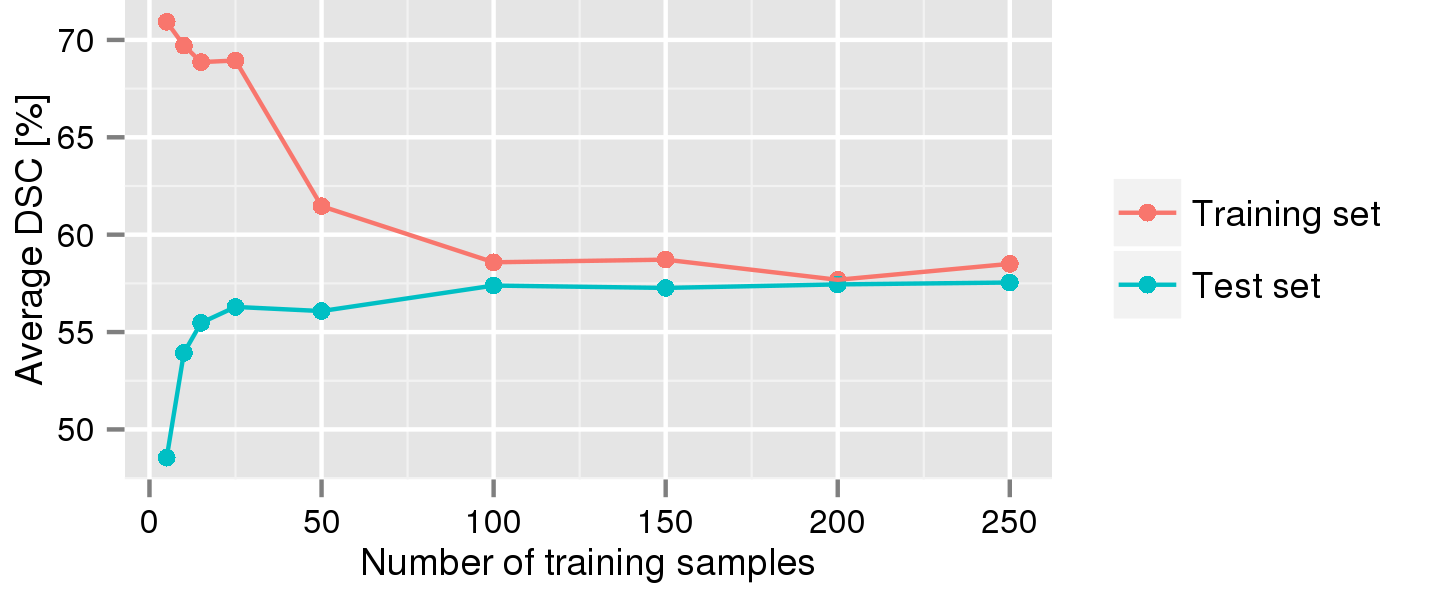
\includegraphics[width=0.78\textwidth]{figures/train_count}

\caption{Comparison of DSC scores calculated on the training and test sets for
varying numbers of training samples. At around 100 samples, the model becomes
stable in terms of test performance and the small difference between training
and test DSCs, indicating that overfitting of the training data no longer
occurs.}
\label{fig:bioms}
\end{figure}
